\documentclass[a4paper]{smallposter}
\geometry{paperwidth=8.5in,paperheight=11in,margin=0in}
\usetikzlibrary{arrows.meta}

\begin{document}

\null\vspace{2cm}
\setfontsize{30}{40}
A Layman's Introduction to \\
\setfontsize{50}{60}
{\bf Quantum Computing}

\vspace{1cm}

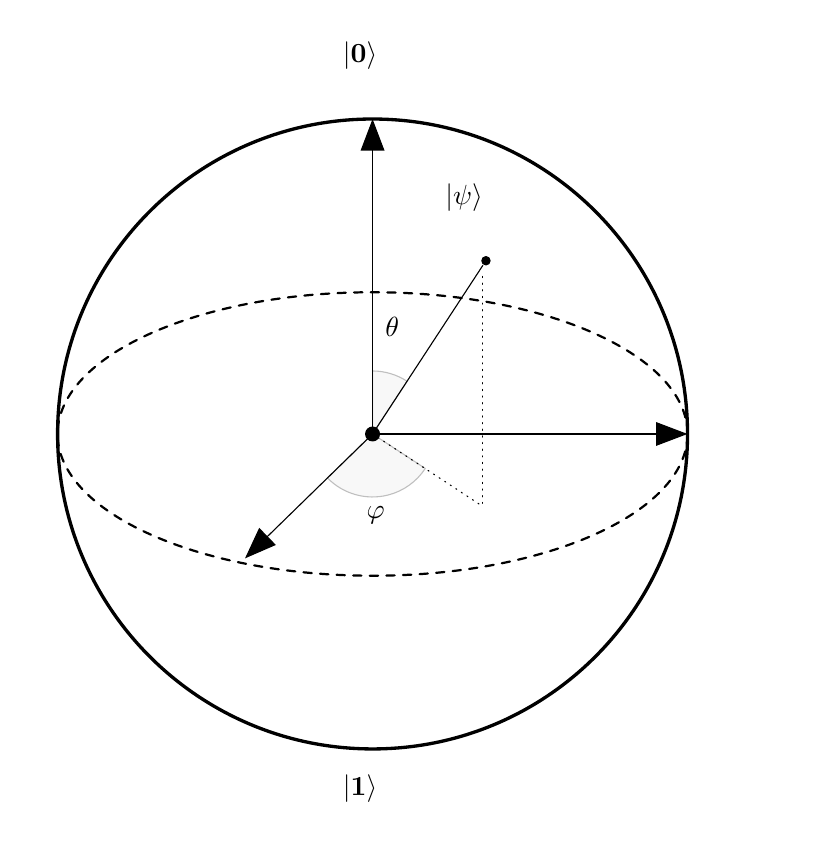
\begin{tikzpicture}[
    line cap=round,
    line join=round,
    >={Triangle[length=4mm,width=3mm]},
    scale=2
  ]
  \setfontsize{14.4}{14.4}
  \clip(-2.19,-2.49) rectangle (2.66,2.58);
  \draw [shift={(0,0)}, lightgray, fill, fill opacity=0.1] (0,0) -- (56.7:0.4) arc (56.7:90.:0.4) -- cycle;
  \draw [shift={(0,0)}, lightgray, fill, fill opacity=0.1] (0,0) -- (-135.7:0.4) arc (-135.7:-33.2:0.4) -- cycle;
  \draw [very thick] (0,0) circle (2cm);
  \draw [thick,rotate around={0.:(0.,0.)},dash pattern=on 3pt off 3pt] (0,0) ellipse (2cm and 0.9cm);
  \draw (0,0)-- (0.70,1.07);
  \draw [->] (0,0) -- (0,2);
  \draw [->] (0,0) -- (-0.81,-0.79);
  \draw [->] (0,0) -- (2,0);
  \draw [dotted] (0.7,1)-- (0.7,-0.46);
  \draw [dotted] (0,0)-- (0.7,-0.46);
  \draw (-0.1,-0.4) node[anchor=north west] {$\varphi$};
  \draw (0.02,0.8) node[anchor=north west] {$\theta$};
  \draw (-0.25,2.55) node[anchor=north west] {$\mathbf {|0\rangle}$};
  \draw (-0.25,-2.1) node[anchor=north west] {$\mathbf {|1\rangle}$};
  \draw (0.4,1.65) node[anchor=north west] {$|\psi\rangle$};
  \draw [fill] (0,0) circle (1.25pt);
  \draw [fill] (0.72,1.1) circle (0.75pt);
\end{tikzpicture}

\vspace{1.25cm}
\setfontsize{25}{30}
I swear you'll understand the basics \\
{\em if it kills me}

\vspace{2.25cm}
\setfontsize{16.5}{24}
UTD Makerspace (SPN 2.222) \\
Thursday, November 21st \\
6:30 - 8pm

\normalsize
\overlayqrcode{south west}{shift={(4cm,3.5cm)}}{height=3cm}{
  https://discord.gg/HA68vVB
}

\overlayimage{north west}{shift={(2cm,-1.25cm)}}{height=1cm}{tux_mono}
\overlaytext{north west}{shift={(4.75cm,-1.25cm)}}{.2\textwidth}{
  \setmainfont{Droid Sans Mono}
  \setfontsize{16}{16}
  OpenUTD
}

\disclaimer{black!50}

\end{document}
